\documentclass[aspectratio  =  169, 15pt]{beamer}
% Strings to reuse

\newcommand{\mydocumenttitle}{Clustering Graphs}
\newcommand{\mydocumentsubtitle}{Applying a Label Propagation Algorithm to Detect Communities in Graph Databases}
\newcommand{\mydocumentfulltitle}{\mydocumenttitle\ - \mydocumentsubtitle}

\newcommand{\mysupervisortitle}{Prof.}
\newcommand{\mysupervisorname}{Stefano}
\newcommand{\mysupervisorsurname}{Paraboschi}
\newcommand{\mysupervisor}{\mysupervisortitle\ \mysupervisorname\ \mysupervisorsurname}

%\newcommand{\myexaminertitle}{Prof.}
%\newcommand{\myexaminername}{ExaminerName}
%\newcommand{\myexaminersurname}{ExaminerSurname}
%\newcommand{\myexaminer}{\myexaminertitle\ \myexaminername\ \myexaminersurname}

\newcommand{\myauthorname}{Name}
\newcommand{\myauthorsurname}{Surname}
\newcommand{\myauthor}{\myauthorname\ \myauthorsurname}
\newcommand{\myauthorregnumber}{0000000}

\newcommand{\myauthoremail}{myaddress@mail.com}
\newcommand{\myauthorgithub}{https://github.com/formidablae}
\newcommand{\myauthorlinkedin}{https://www.linkedin.com/in/abcde}

\newcommand{\mydocumentsubject}{Master’s Thesis}
\newcommand{\mycourse}{Master’s Degree in Computer Science \& Engineering}
\newcommand{\myinstitution}{University of Bergamo}
\newcommand{\myinstitutiondepartment}{School of Engineering}
\newcommand{\myinstitutionaddress}{Viale G. Marconi, 5,\\24044\\Dalmine, BG\\Italy}
\newcommand{\myinstitutionaddressinline}{Viale G. Marconi, 5, 24044 Dalmine, BG, Italy}
\newcommand{\myplaceofpublishing}{Bergamo, Italy}

\newcommand{\mydayofpublishing}{23}
\newcommand{\mymonthofpublishing}{09}
\newcommand{\myyearofpublishing}{2021}
\newcommand{\mydateofpublishing}{\myyearofpublishing-\mymonthofpublishing-\mydayofpublishing}% do not use comma between month and year
\newcommand{\mykeywords}{Detecting, communities, graphs, Graph, Databases, Graph Databases, thesis, master, master's thesis, academia, computer engineering, computer science, \myauthor, \mysupervisor, unibg, Università degli Studi di Bergamo, University of Bergamo}
\definecolor{white}{rgb}{1,1,1}
\definecolor{whitesmoke}{rgb}{0.985,0.985,0.985}
\definecolor{whitedarksmoke}{rgb}{0.965,0.965,0.965}
\definecolor{lightestgray}{rgb}{0.95,0.95,0.95}
\definecolor{lightstgray}{rgb}{0.90,0.90,0.90}
\definecolor{lightergray}{rgb}{0.85,0.85,0.85}
\definecolor{lightlightergray}{rgb}{0.80,0.80,0.80}
\definecolor{lightgray}{rgb}{0.75,0.75,0.75}
\definecolor{lghtgray}{rgb}{0.6,0.6,0.6}
\definecolor{gray}{rgb}{0.5,0.5,0.5}
\definecolor{dkgray}{rgb}{0.45,0.45,0.45}
\definecolor{darkgray}{rgb}{0.35,0.35,0.35}
\definecolor{darkergray}{rgb}{0.27,0.27,0.27}
\definecolor{darkestgray}{rgb}{0.15,0.15,0.15}
\definecolor{blacksmoke}{rgb}{0.05,0.05,0.05}
\definecolor{black}{rgb}{0,0,0}

\definecolor{moderngreen}{rgb}{0.13, 0.34, 0.48}
\definecolor{darkgreen}{rgb}{0,0.6,0}
\definecolor{darkergreen}{rgb}{0,0.4,0}
\definecolor{lightgreen}{rgb}{0,0.9,0}
\definecolor{darkpurple}{rgb}{0.65, 0.12, 0.82}
\definecolor{goldenyellow}{rgb}{1.0, 0.84, 0.0}
\definecolor{mauve}{rgb}{0.58,0,0.82}
\definecolor{lightblue}{rgb}{0.0,0.0,0.9}
\definecolor{darkblue}{rgb}{0.0,0.0,0.6}
\definecolor{cyan}{rgb}{0.0,0.6,0.6}
\definecolor{darkred}{rgb}{0.6,0.0,0.0}
\definecolor{royalblue}{rgb}{0.25,0.41,0.88}

\usetheme[
    progressbar  =  frametitle,% progress bar of slides. Can be none, head, frametitle, foot
    titleformat title  =  regular,% can be regular, smallcaps, allsmallcaps, allcaps
    titleformat subtitle  =  regular,% can be regular, smallcaps, allsmallcaps, allcaps
    titleformat section  =  regular,% can be regular, smallcaps, allsmallcaps, allcaps
    titleformat frame  =  regular,% can be regular, smallcaps, allsmallcaps, allcaps
    sectionpage  =  simple,% can be none, simple, progressbar
    subsectionpage  =  none,% can be none, simple, progressbar
    numbering  =  none,% for slide numbers can be none, counter, fraction
    background  =  light% for slides and text dark light contrasts. Can be light or dark
]{metropolis}

\hyphenpenalty = 10000% no hyphenation in presentation

\usepackage{hyperref}
\hypersetup{
    bookmarksopen = true,
    bookmarksopenlevel=4,
    pdfstartview={Fit},
    pdfpagemode=FullScreen,
    pdffitwindow=true,
    breaklinks = true,% to correctly break links
    pdftitle = {\mydocumentfulltitle\ (\myauthor)},
    pdfauthor = {\myauthor},
    pdfsubject = {\mydocumentfulltitle},
    pdfcreator = {\myauthor},
    pdfproducer = {\myauthor},
    pdfkeywords = {\mykeywords}
}

\setsansfont{Roboto}% text font
\setmonofont{Roboto Mono}% monospace text font

\setbeamercolor{normal text}{
    fg = darkgray,% frame text color
    bg  = whitesmoke% frame background color
}
\setbeamercolor{palette primary}{
    fg  =  whitesmoke,% standout frame text color
    bg  =  moderngreen% standout frame background color
}
\setbeamercolor{alerted text}{fg = darkgray}
\setbeamercolor{frametitle}{
    fg  =  whitesmoke,% frame title text color
    bg  =  moderngreen% frame title background color
}
\setbeamercolor{progress bar}{
    fg  =  goldenyellow,% progress bar text color
    bg  =  moderngreen% progress bar background color
}

\usepackage{booktabs}% good looking tables. Allows the use of \toprule, \midrule and \bottomrule in tables
\usepackage{multicol}% text in multiple columns, useful for side-by-side text and pictures

\usepackage{tikz}
\usetikzlibrary{backgrounds,calc}

%%%%% notes %%%%%
\usepackage{pgfpages}
%\setbeameroption{hide notes}% Show only slides
%\setbeameroption{show only notes}% Show only notes
\setbeameroption{show notes on second screen=bottom}% Show notes and slides
\setbeamerfont{note page}{size=\large}
\setbeamertemplate{itemize/enumerate subbody begin}{\large}
%%%%%%%%%%%%%%%%%

\begin{document}
    \begin{frame}{}
        \begin{tikzpicture}[remember picture,overlay]
            \begin{pgfonlayer}{background}
                \node[anchor=south east,outer sep=0pt,inner sep=0pt] at ($(current page.south east) +(-0in,0in)$) {
                    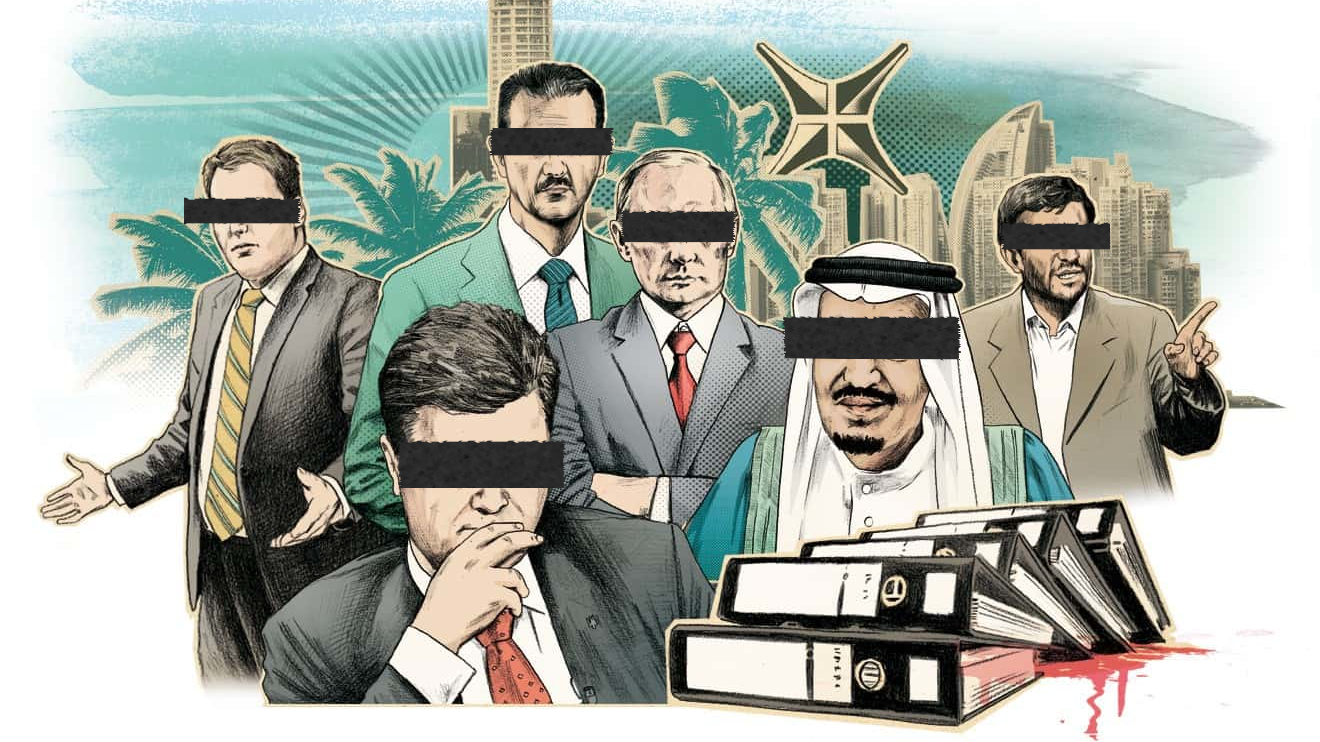
\includegraphics[width = 1\paperwidth, height = 1\paperheight, keepaspectratio]{images/panamapapers/coverpanamapapershidden.jpg}
                };
            \end{pgfonlayer}
        \end{tikzpicture}
        \note[item]{
            Qualcuno saprebbe riconoscere chi sono le persone in questa slide?
        
            {\color{orange}\textit{wait 5 seconds}}
        }
        \note[item]{
            Vediamolo:
            
            {\color{blue}\textit{go to next slide}}
        }
    \end{frame}
    
    \begin{frame}{}
        \begin{tikzpicture}[remember picture,overlay]
            \begin{pgfonlayer}{background}
                \node[anchor=south east,outer sep=0pt,inner sep=0pt] at ($(current page.south east) +(-0in,0in)$) {
                    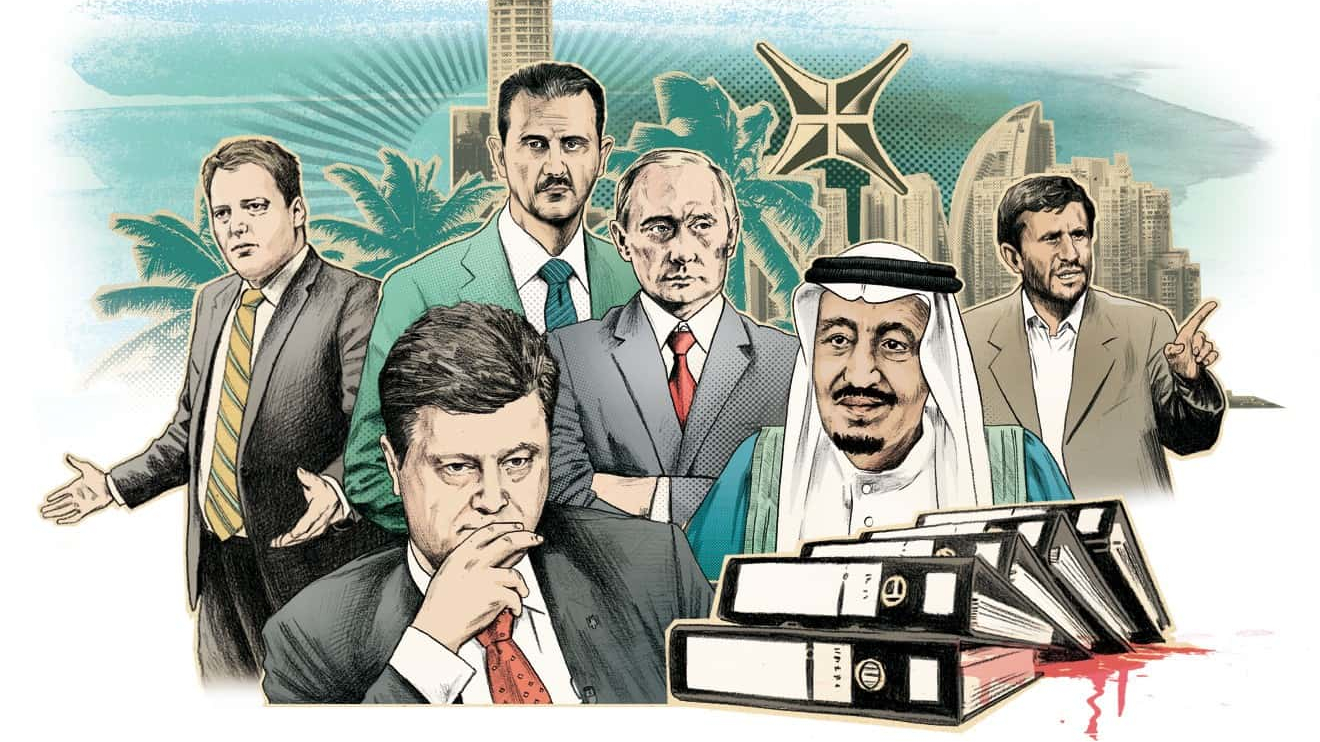
\includegraphics[width = 1\paperwidth, height = 1\paperheight, keepaspectratio]{images/panamapapers/coverpanamapapersrevealed.jpg}
                };
            \end{pgfonlayer}
        \end{tikzpicture}
        \note[item]{
            Putin, Assad, Poroshenko, il re Salman, Ahmadinejad...
            
            Tutti politici di altissimo livello...
        }
        \note[item]{
            che appaiono nel...
            
            {\color{blue}\textit{go to next slide}}
        }
    \end{frame}
    
    \begin{frame}{}
        \begin{tikzpicture}[remember picture,overlay]
            \begin{pgfonlayer}{background}
                \node[anchor=south east,outer sep=0pt,inner sep=0pt] at ($(current page.south east) +(-0in,0in)$) {
                    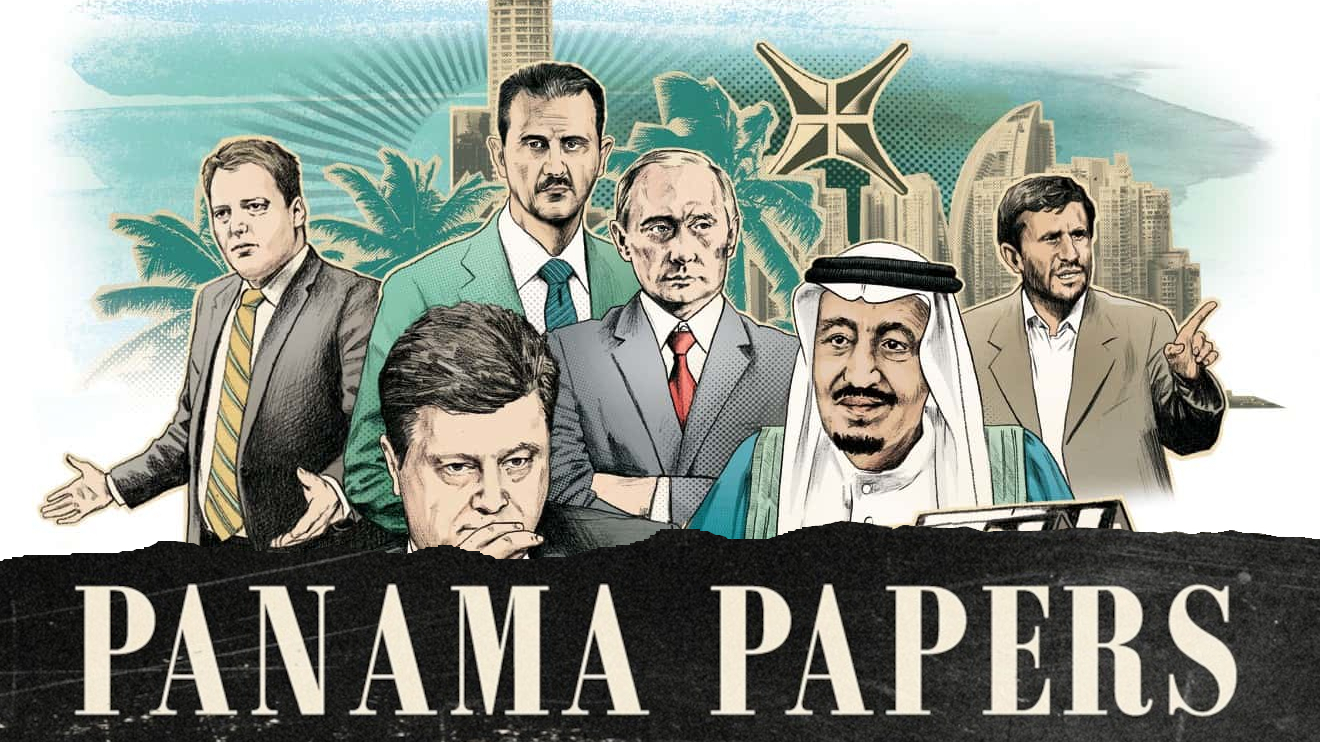
\includegraphics[width = 1\paperwidth, height = 1\paperheight, keepaspectratio]{images/panamapapers/coverpanamapapersrevealedtitled.jpg}
                };
            \end{pgfonlayer}
        \end{tikzpicture}
        \note[item]{
            ...Panama Papers leak.
        }
        \note[item]{
            Ma cosa era Panama Papers?
            
            {\color{blue}\textit{go to next slide}}
        }
    \end{frame}
    
    \begin{frame}{}
        \begin{tikzpicture}[remember picture,overlay]
            \begin{pgfonlayer}{background}
                \node[anchor=south east,outer sep=0pt,inner sep=0pt] at ($(current page.south east) +(-0in,0in)$) {
                    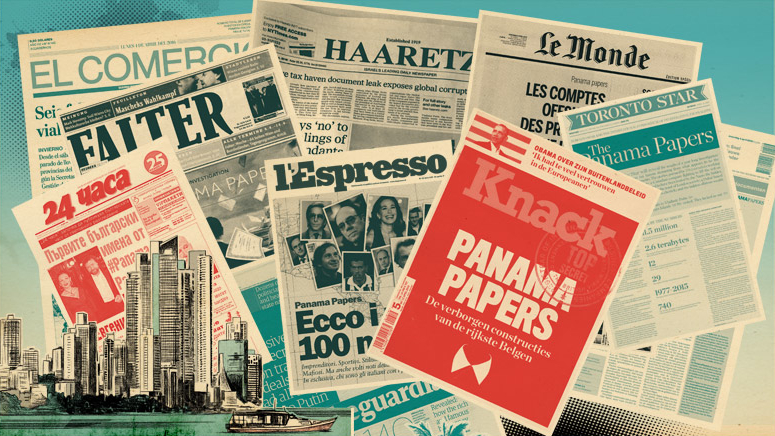
\includegraphics[width = 1\paperwidth, height = 1\paperheight, keepaspectratio]{images/panamapapers/newspapers.jpg}
                };
            \end{pgfonlayer}
        \end{tikzpicture}
        \note[item]{
            \begin{itemize}
                \item In aprile 2016,
                \item grazie ad un informatore,
                \item l'inchiesta di 307 giornalisti da 76 paesi ha portato alla luce documenti e informazioni
                \item su migliardi di denaro dirottati da studi legali internazionali e banche verso paradisi fiscali
                \item per conto di...
            \end{itemize}
            
            {\color{blue}\textit{go to next slide}}
        }
    \end{frame}
    
    \begin{frame}{}
        \begin{tikzpicture}[remember picture,overlay]
            \begin{pgfonlayer}{background}
                \node[anchor=south east,outer sep=0pt,inner sep=0pt] at ($(current page.south east) +(-0in,0in)$) {
                    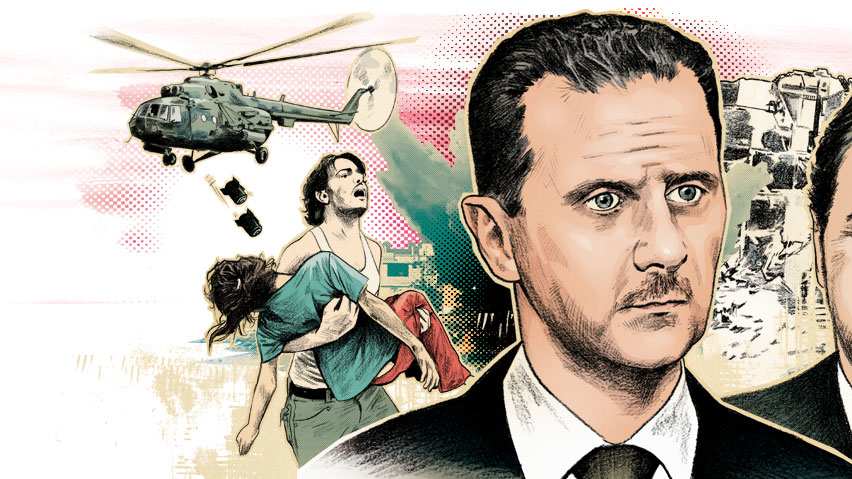
\includegraphics[width = 1\paperwidth, height = 1\paperheight, keepaspectratio]{images/panamapapers/Assad.jpg}
                };
            \end{pgfonlayer}
        \end{tikzpicture}
        \note[item]{
            ... leader politici, criminali ...
            
            {\color{blue}\textit{go to next slide}}
        }
    \end{frame}
    
    \begin{frame}{}
        \begin{tikzpicture}[remember picture,overlay]
            \begin{pgfonlayer}{background}
                \node[anchor=south east,outer sep=0pt,inner sep=0pt] at ($(current page.south east) +(-0in,0in)$) {
                    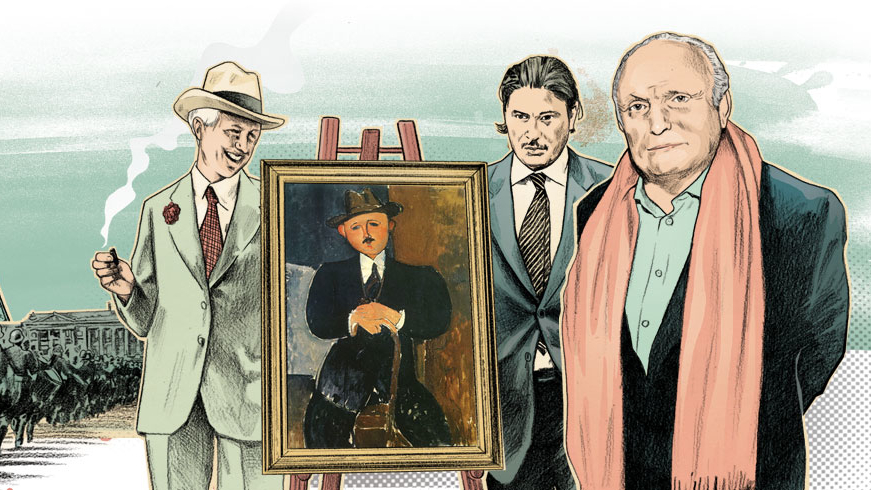
\includegraphics[width = 1\paperwidth, height = 1\paperheight, keepaspectratio]{images/panamapapers/art.jpg}
                };
            \end{pgfonlayer}
        \end{tikzpicture}
        \note[item]{
            ... funzionari d'intelligence, artisti ...
            
            {\color{blue}\textit{go to next slide}}
        }
    \end{frame}
    
    \begin{frame}{}
        \begin{tikzpicture}[remember picture,overlay]
            \begin{pgfonlayer}{background}
                \node[anchor=south east,outer sep=0pt,inner sep=0pt] at ($(current page.south east) +(-0in,0in)$) {
                    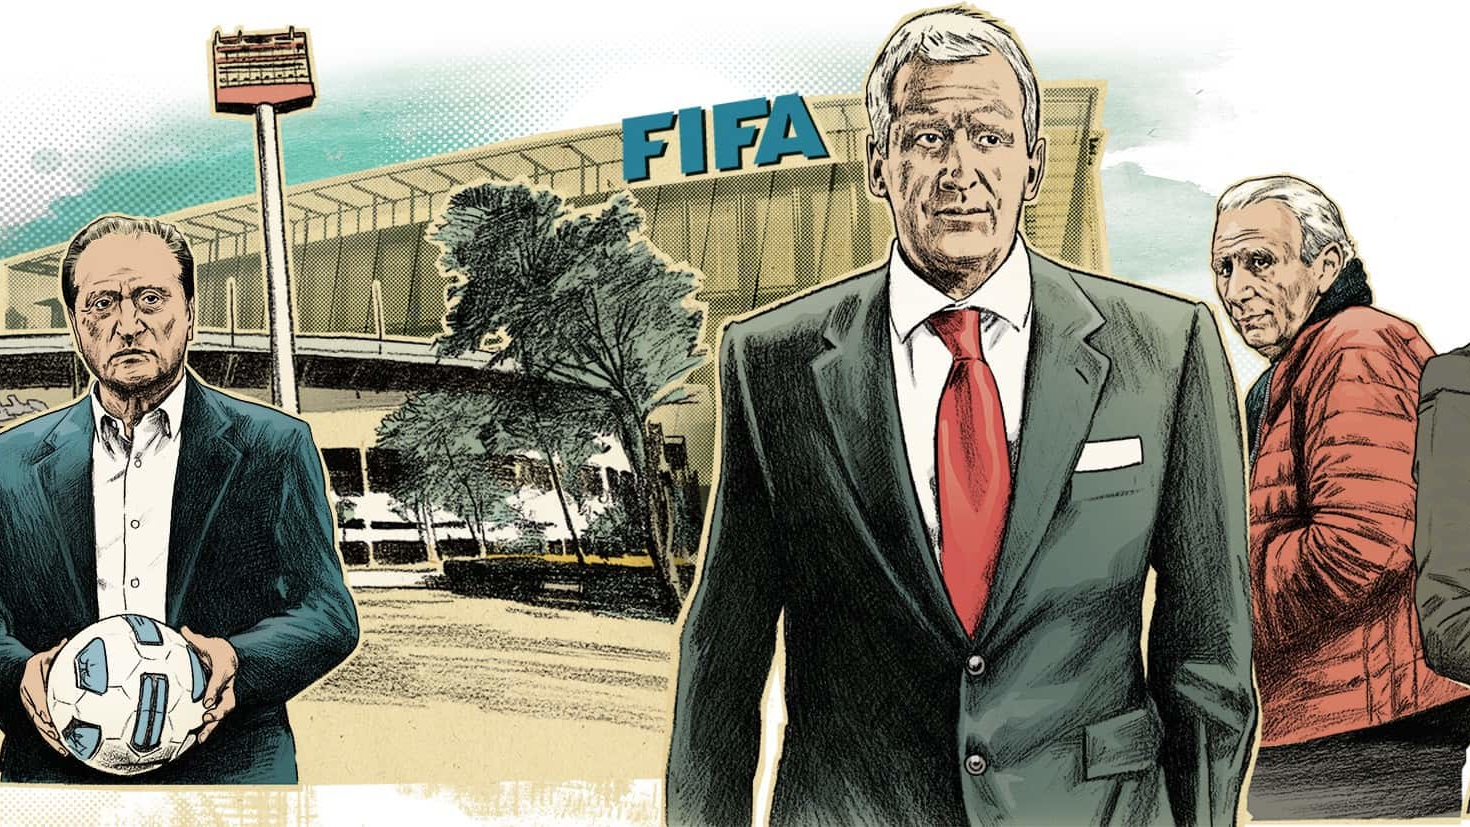
\includegraphics[width = 1\paperwidth, height = 1\paperheight, keepaspectratio]{images/panamapapers/FIFA1.jpg}
                };
            \end{pgfonlayer}
        \end{tikzpicture}
        \note[item]{
            ... VIP dello sport ...
            
            {\color{blue}\textit{go to next slide}}
        }
    \end{frame}
    
    \begin{frame}{}
        \begin{tikzpicture}[remember picture,overlay]
            \begin{pgfonlayer}{background}
                \node[anchor=south east,outer sep=0pt,inner sep=0pt] at ($(current page.south east) +(-0in,0in)$) {
                    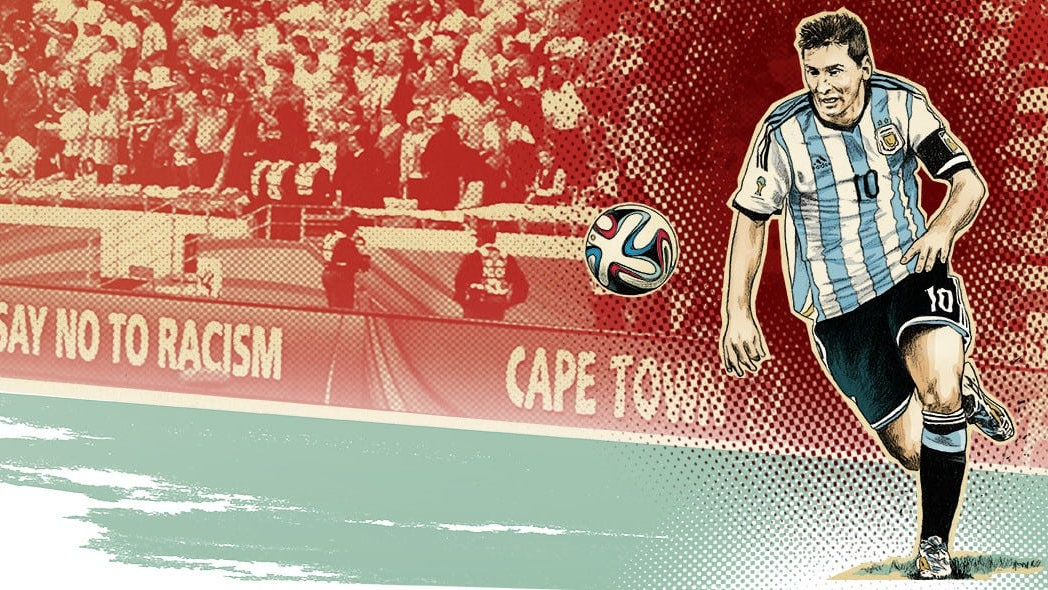
\includegraphics[width = 1\paperwidth, height = 1\paperheight, keepaspectratio]{images/panamapapers/Messi.jpg}
                };
            \end{pgfonlayer}
        \end{tikzpicture}
        \note[item]{
            ... e dello spettacolo.
            
            {\color{orange}\textit{wait 5 seconds}}
        }
        \note[item]{
            \begin{itemize}
                \item Quanto era grande il dataset leakato?
                \item ... come erano strutturati i dati?
            \end{itemize}
            
            {\color{blue}\textit{go to next slide}}
        }
    \end{frame}
    
    \begin{frame}{}
        \begin{tikzpicture}[remember picture,overlay]
            \begin{pgfonlayer}{background}
                \node[anchor=south east,outer sep=0pt,inner sep=0pt] at ($(current page.south east) +(-0in,0in)$) {
                    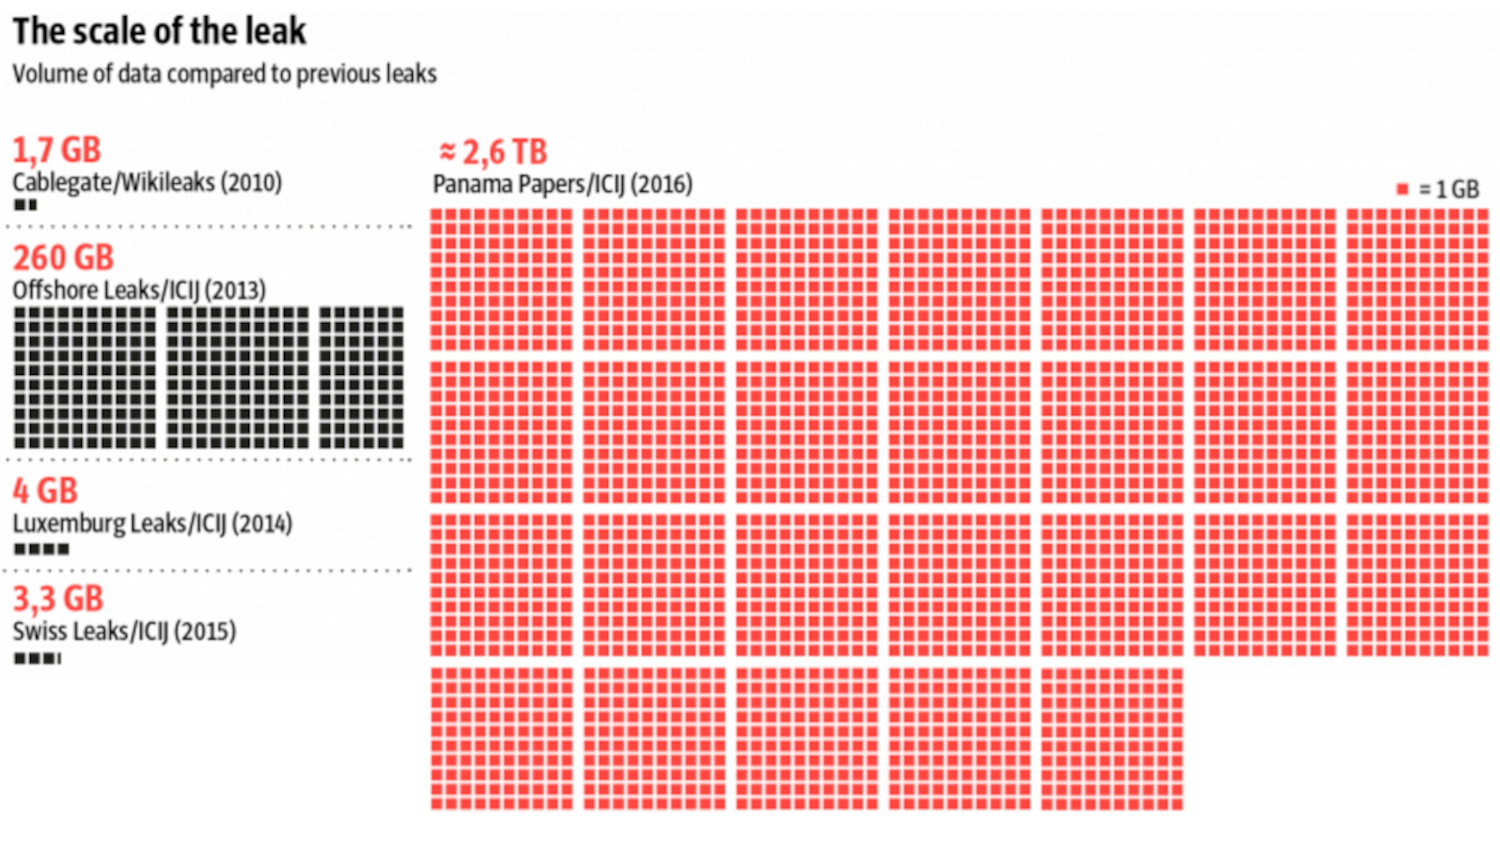
\includegraphics[width = 1\paperwidth, height = 1\paperheight, keepaspectratio]{images/panamapapers/datasetsizenew.jpg}
                };
            \end{pgfonlayer}
        \end{tikzpicture}
        \note[item]{
            Il leak era di dimensione 2.6 TB, 1500 volte più grande del Cablegate del 2010 di Wikileaks.
            
            {\color{blue}\textit{go to next slide}}
        }
    \end{frame}
    
    \begin{frame}{}
        \begin{tikzpicture}[remember picture,overlay]
            \begin{pgfonlayer}{background}
                \node[anchor=south east,outer sep=0pt,inner sep=0pt] at ($(current page.south east) +(-0in,0in)$) {
                    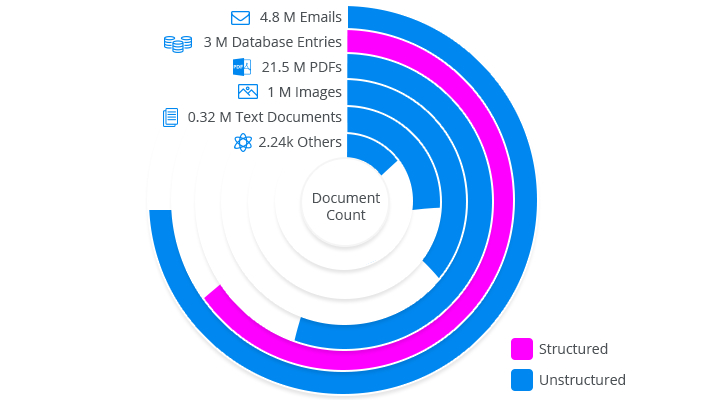
\includegraphics[width = 1\paperwidth, height = 1\paperheight, keepaspectratio]{images/panamapapers/datatypes.jpg}
                };
            \end{pgfonlayer}
        \end{tikzpicture}
        \note[item]{
            La maggior parte dei dati erano non strutturati, sotto forma di email, files PDF e immagini inviati.
            
            {\color{blue}\textit{go to next slide}}
        }
    \end{frame}
    
    \begin{frame}{}
        \begin{tikzpicture}[remember picture,overlay]
            \begin{pgfonlayer}{background}
                \node[anchor=south east,outer sep=0pt,inner sep=0pt] at ($(current page.south east) +(-0in,0in)$) {
                    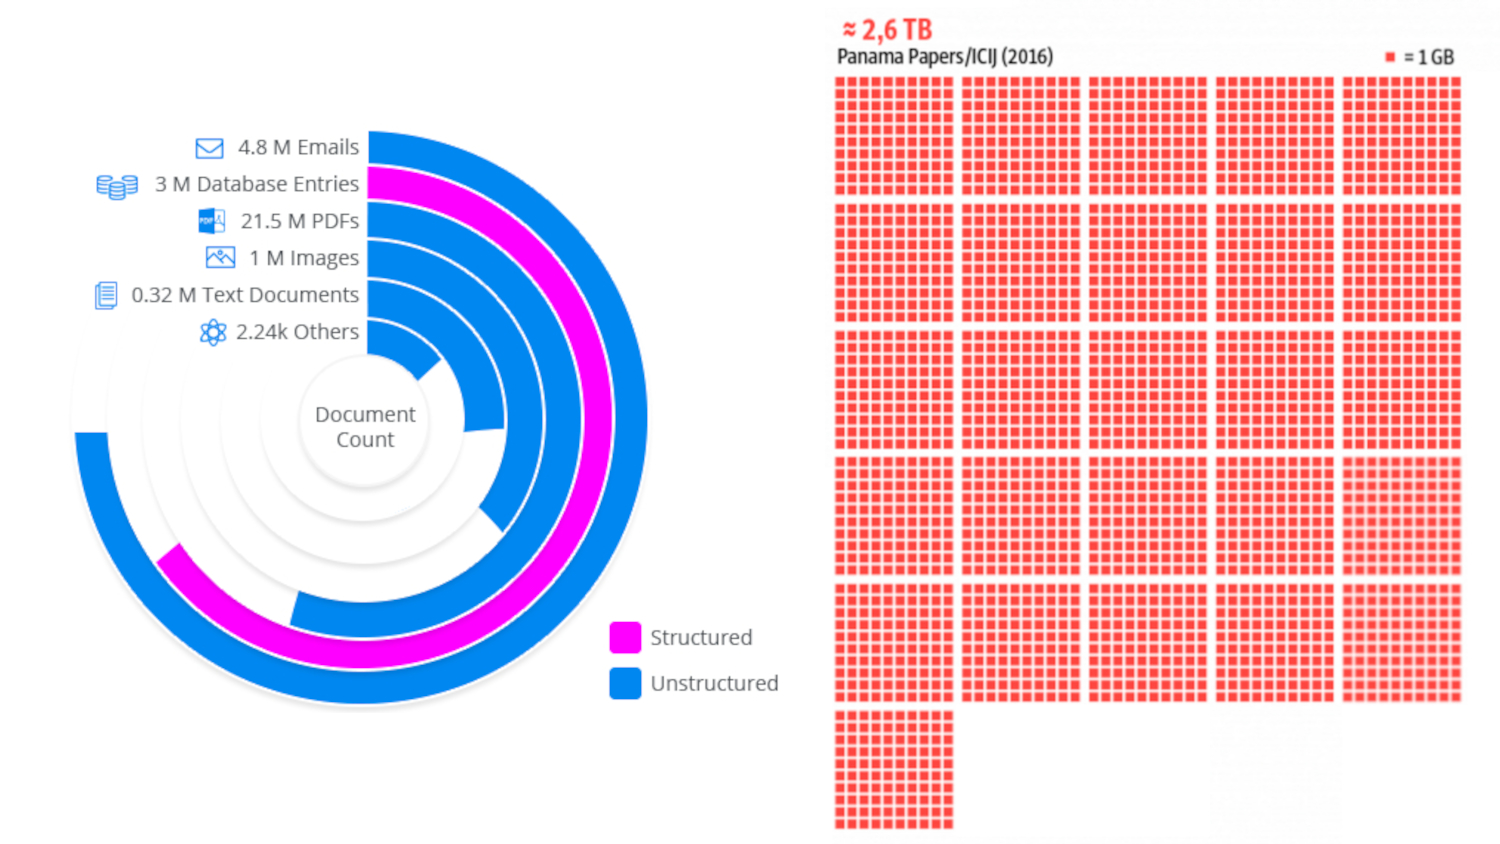
\includegraphics[width = 1\paperwidth, height = 1\paperheight, keepaspectratio]{images/panamapapers/datasetsizeandtypes.jpg}
                };
            \end{pgfonlayer}
        \end{tikzpicture}
        \note[item]{
            Come si può indagare su un dataset così immenso e in gran parte fatto di dati non strutturati?
            
            {\color{blue}\textit{go to next slide}}
        }
    \end{frame}
    
    \begin{frame}{}
        \begin{tikzpicture}[remember picture,overlay]
            \begin{pgfonlayer}{background}
                \node[anchor=south east,outer sep=0pt,inner sep=0pt] at ($(current page.south east) +(-0in,0in)$) {
                    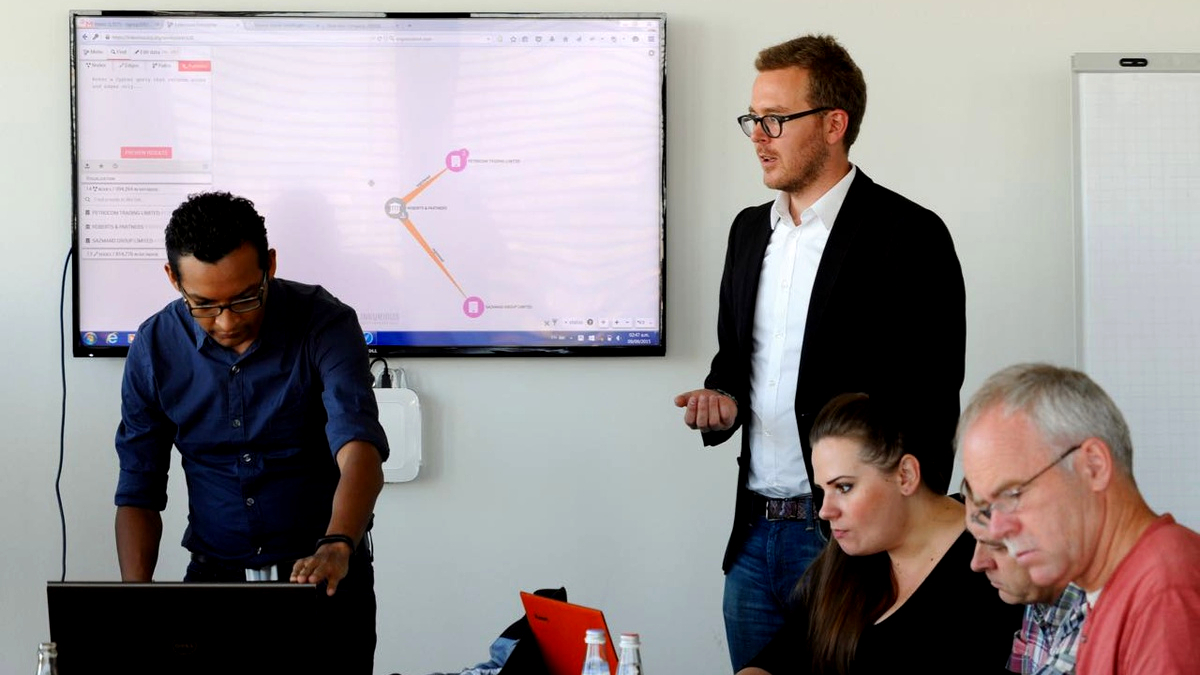
\includegraphics[width = 1\paperwidth, height = 1\paperheight, keepaspectratio]{images/panamapapers/team.jpg}
                };
            \end{pgfonlayer}
        \end{tikzpicture}
        \note[item]{
            Loro, un team composto da giornalisti investigativi ed esperti di database a grafi ce l'hanno fatta.
        }
        \note[item]{
            Facendo buon uso delle relazioni che derivano da dati interconnessi (ad esempio le mail, le dipendenze tra le entità) ...
            
            {\color{blue}\textit{go to next slide}}
        }
    \end{frame}
    
    \begin{frame}{}
        \begin{tikzpicture}[remember picture,overlay]
            \begin{pgfonlayer}{background}
                \node[anchor=south east,outer sep=0pt,inner sep=0pt] at ($(current page.south east) +(-0in,0in)$) {
                    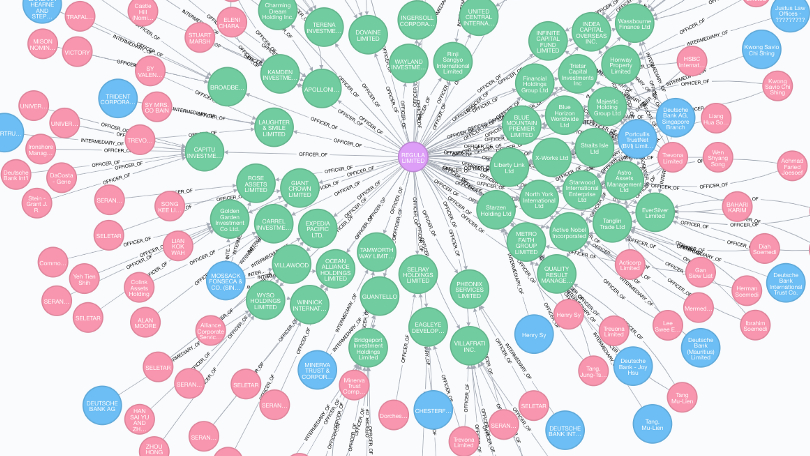
\includegraphics[width = 1\paperwidth, height = 1\paperheight, keepaspectratio]{images/panamapapers/graph.jpg}
                };
            \end{pgfonlayer}
        \end{tikzpicture}
        \note[item]{
            \begin{itemize}
                \item ... e di nuove tecnologie (come i database a grafi),
                \item hanno generato grafi rappresentanti le entità e le connessioni tra loro,
                \item interrogabili
            \end{itemize}
            
            {\color{blue}\textit{go to next slide}}
        }
    \end{frame}
    
    \begin{frame}[noframenumbering,standout]
        \normalfont
        
        \vspace*{0.75cm}
        \fontsize{26pt}{33pt}\selectfont\textsc{\break\mydocumenttitle}
        
        \begin{columns}[t]
            \column{0.13\textwidth}
            
            \column{0.69\textwidth}
                \vspace*{-1.25cm}
                \begin{center}
                    \Large\normalfont\mydocumentsubtitle
                    
                    \vspace*{0.5cm}
                    \normalsize\textbf{\myauthor}
                \end{center}
                
                    
                %\mydateofpublishing
                
                \begin{tikzpicture}[remember picture,overlay]
                    \begin{pgfonlayer}{background}
                        \node[anchor=south east,outer sep=0pt,inner sep=0pt] at ($(current page.south east) +(-0in,0in)$) {
                            
\includegraphics[width = 0.25\paperwidth]{images/LogoUniBGwhiterotatedcut.pdf}
                        };
                    \end{pgfonlayer}
                \end{tikzpicture}
                
            \column{0.13\textwidth}
        \end{columns}
    \end{frame}
    
    \section{What are graphs?}
    
    \begin{frame}{Milan Metro subway stations and lines (vertices and edges)}
        \centering
        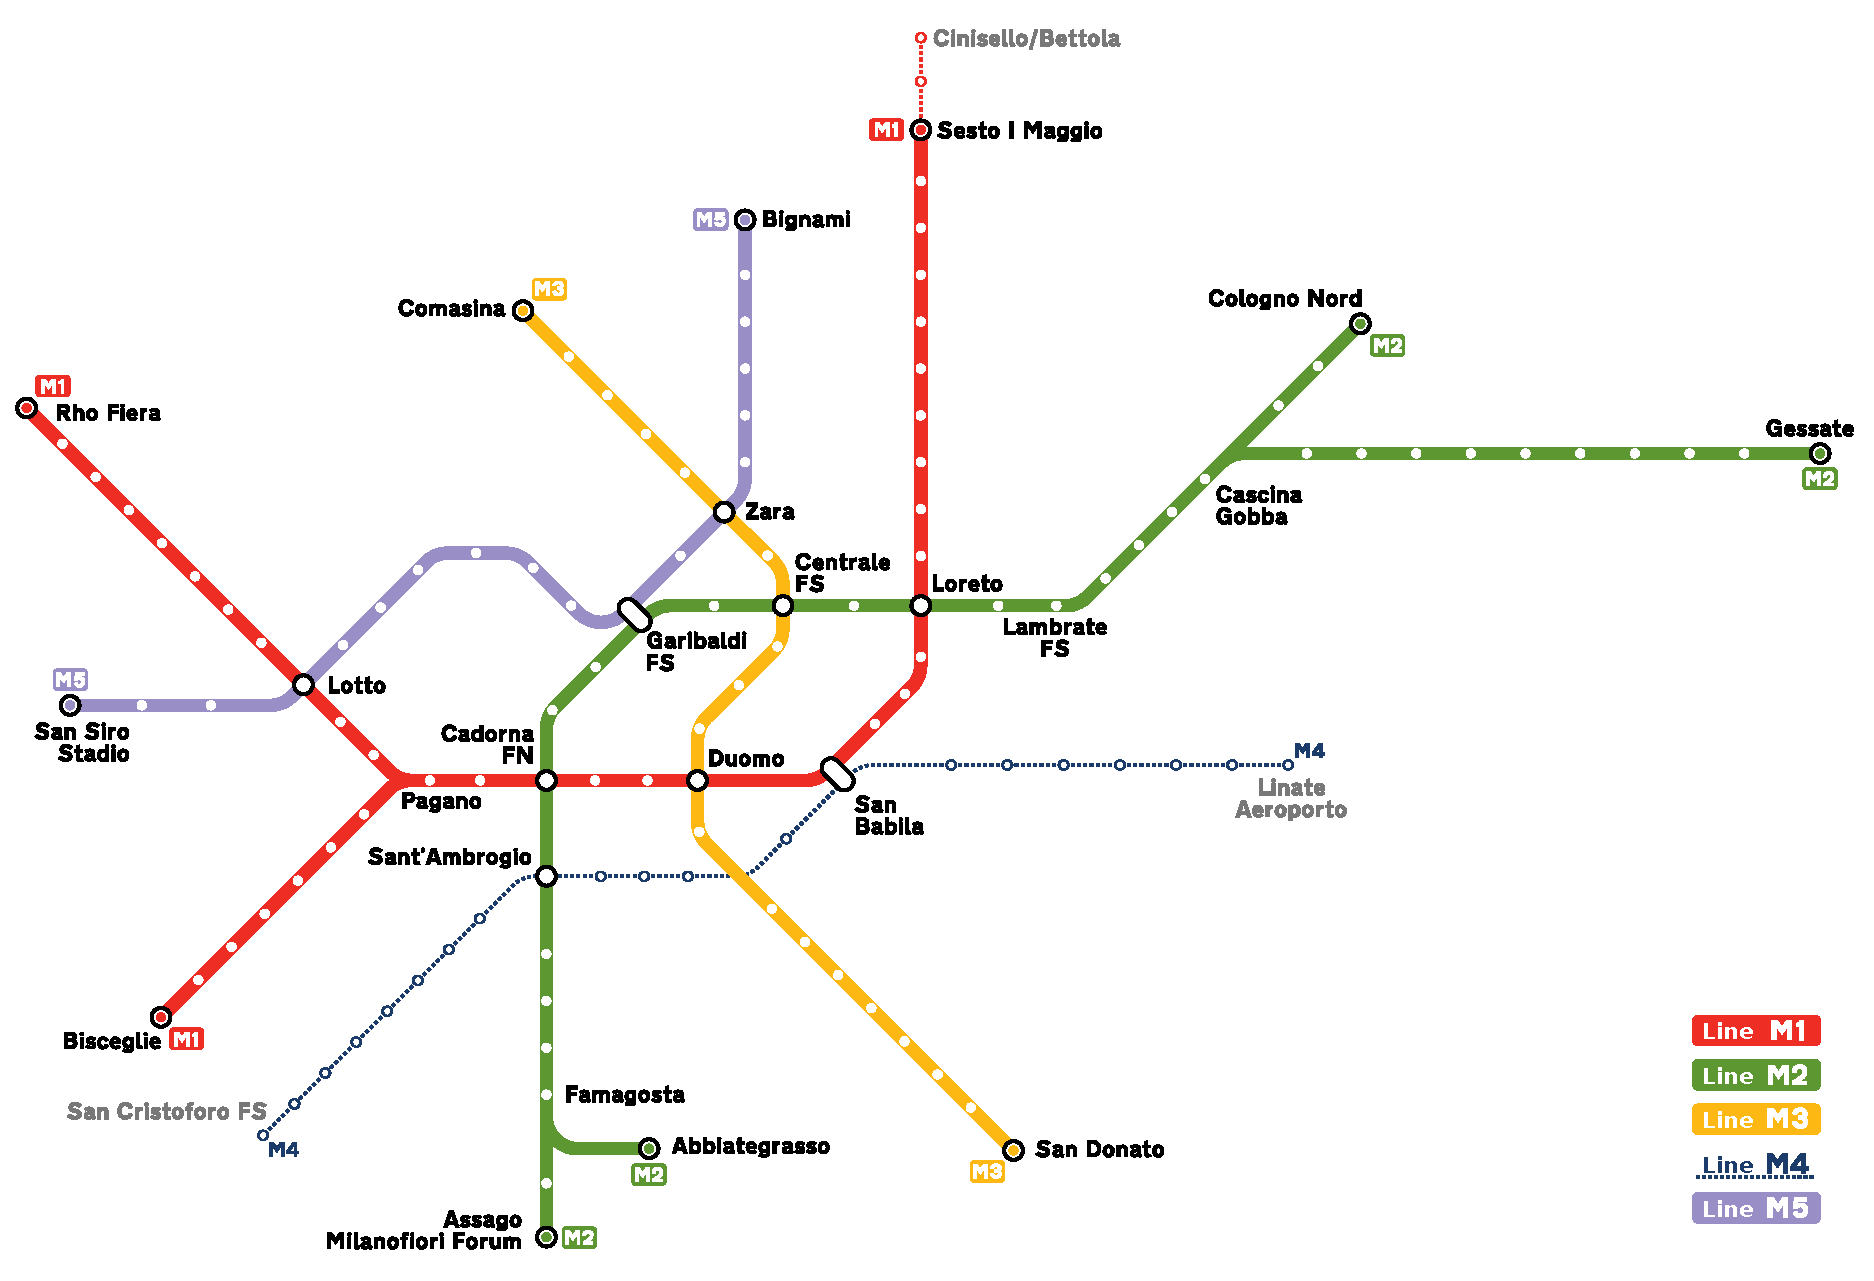
\includegraphics[width = 0.78\paperwidth, height = 0.78\paperheight, keepaspectratio]{images/ch2/WikipediaMilanoMetro2021Graphedit.pdf}
    \end{frame}
    
    \section{What about graph databases?}
    
    \begin{frame}{Database types ordered by complexity of data}
        \centering
        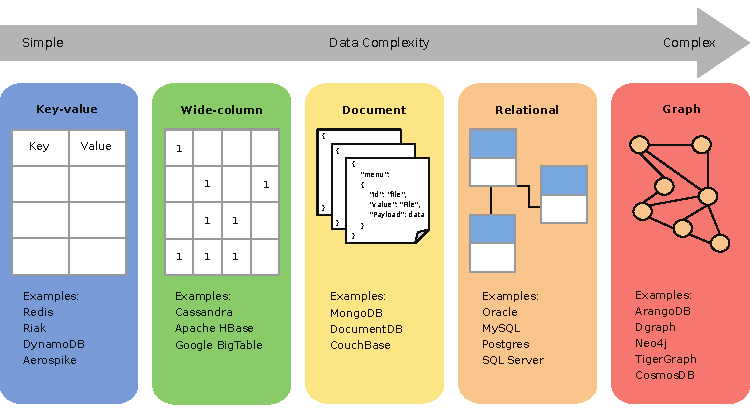
\includegraphics[width = 0.78\paperwidth, height = 0.78\paperheight, keepaspectratio]{images/ch1/BechbergerPerryman2020page8.pdf}
    \end{frame}
    
    
    \begin{frame}{Your Title}
        nsectetuer adipiscing elit.Ut purus elit, vestibulum ut, placerat ac, adipiscing vitae,felis. Curabitur dictum gravida mauris. Nam arcu libero,nonummy eget, consectetuer id, vulputate a,
        
        \begin{itemize}
        	\item che mostrino l'{\color{mauve}Albero Sintattico},
        	\item che stampino la {\color{orange}Tabella dei Simboli},
        	\item e che nello stesso tempo facciano da {\color{blue}Compilatore}.
        \end{itemize}
    \end{frame}
    
    \section{2 Section}
    
    \begin{frame}{Your Title}
        Lorem ipsum dolor sit amet, conse purus elit, vestibulum ut, placerat ac, adipiscing vitae,felis. Curabitur dictum gravida mauris. Nam arcu libero,nonummy eget, consectetuer id, vulputate a,
        \begin{columns}[t]
        \column{.30\textwidth}
            \begin{itemize}
            	\item vedere ed esportare l'{\color{yellow}Albero Sintattico} del parsing di un programma
            \end{itemize}
            \column{.67\textwidth}
            \vspace*{-25pt}
            \begin{figure}[H]
                \centering
                \noindent\makebox[\textheight]{
                    
\includegraphics[
                        width=0.5\paperwidth,
                        height=0.5\paperheight,
                        keepaspectratio
                    ]{images/LogoUniBGwhiterotatedcut.pdf}
                }
            \end{figure}
        \end{columns}
    \end{frame}
    
    \begin{frame}{Your Title}
        Lorem ipsum dolor sit amet, consectetuer adipiscing elit.Ut t, placerat ac, adipiscing vitae,felis. Curabitur dictum gravida mauris. Nam arcu libero,nonummy eget, consectetuer id, vulputate a,
    \end{frame}
    
    \section{3 Section}
    
    \begin{frame}{Your Title}
        Lorem ipsum dolor sit amet, consectetuer adipiscing elit.Ut purus elit, vestibulum ut, placerat ac, adipiscing vitae,felis. Curabitur
    \end{frame}
    
    \begin{frame}
    \setbeamertemplate{background}{red}
        Lorem ipsum dolor sit amet, consectetuer adipiscing elit.Ut purus elit, vestibulum ut, placerat ac, adipiscing vitae,felis. Curabitur
    \end{frame}
    
    
    \begin{frame}[standout]
        \normalfont
        \vspace*{2.25cm}
        \Huge Thank you!
        
        \vspace*{0.625cm}
        Questions?
        \vspace*{0.125cm}
        \begin{columns}[t]
            \column{.08\textwidth}
            
            \column{.17\textwidth}
                \vspace*{0.2cm}
                \centering\normalsize\break\myauthor
                
            \column{.25\textwidth}
                \vspace*{-0.9cm}
                \begin{flushright}
                    \large\textbf{\textsc{\break\mydocumenttitle}}
                \end{flushright}
                
            \column{.315\textwidth} \scriptsize\normalfont\break\mydocumentsubtitle
                
            \column{.10\textwidth}
        \end{columns}
    \end{frame}

\end{document}
